\documentclass[11pt,a4paper]{article}

% ── Packages ──────────────────────────────────────────────────────────────────
\usepackage[a4paper, top=2.5cm, bottom=2.5cm, left=2.5cm, right=2.5cm]{geometry}
\usepackage[T1]{fontenc}
\usepackage[utf8]{inputenc}
\usepackage{lmodern}
\usepackage[english]{babel}
\usepackage{microtype}
\usepackage{graphicx}
\usepackage{float}
\usepackage{booktabs}
\usepackage{tabularx}
\usepackage{multirow}
\usepackage{xcolor}
\usepackage{hyperref}
\usepackage{amsmath}
\usepackage{enumitem}
\usepackage{caption}
\usepackage{subcaption}
\usepackage{parskip}
\usepackage{titlesec}
\usepackage{fancyhdr}
\usepackage{setspace}
\usepackage{listings}
\usepackage{array}
\usepackage{colortbl}
\usepackage[above,below]{placeins}

% ── Typography ─────────────────────────────────────────────────────────────────
\setstretch{1.07}
\setlength{\parskip}{5pt}
\captionsetup{font=small, labelfont=bf}

\titleformat{\section}{\large\bfseries}{\thesection}{1em}{}
\titleformat{\subsection}{\normalsize\bfseries}{\thesubsection}{1em}{}
\titleformat{\subsubsection}{\normalsize\itshape}{\thesubsubsection}{1em}{}
\titlespacing{\section}{0pt}{10pt}{4pt}
\titlespacing{\subsection}{0pt}{6pt}{2pt}
\titlespacing{\subsubsection}{0pt}{4pt}{1pt}

% ── Header / footer ───────────────────────────────────────────────────────────
\pagestyle{fancy}
\fancyhf{}
\rhead{\small GEMA $\cdot$ CC3051 $\cdot$ 2025/26}
\lhead{\small Mariana Bissacot}
\cfoot{\thepage}
\renewcommand{\headrulewidth}{0.4pt}

% ── Hyperref ──────────────────────────────────────────────────────────────────
\hypersetup{
  colorlinks=true, linkcolor=blue!60!black,
  citecolor=blue!60!black, urlcolor=blue!60!black,
  pdftitle={GEMA: Gender Evolution in Multimodal Archives},
  pdfauthor={Mariana Bissacot},
}

% ── Listings style ────────────────────────────────────────────────────────────
\lstset{
  basicstyle=\ttfamily\footnotesize,
  breaklines=true, frame=single,
  numbers=left, numberstyle=\tiny,
  captionpos=b, xleftmargin=1.5em
}

\definecolor{lightgray}{gray}{0.93}

% ══════════════════════════════════════════════════════════════════════════════
\begin{document}
% ══════════════════════════════════════════════════════════════════════════════

% ── Cover page ────────────────────────────────────────────────────────────────
\begin{titlepage}
  \centering
  \vspace*{1cm}
  {\Large\bfseries Faculdade de Ciências da Universidade do Porto\\}
  \vspace{0.3cm}
  {\large Departamento de Ciência de Computadores\\}
  \vspace{0.3cm}
  {\normalsize CC3051 — Estágio / Projeto $\cdot$ 2025/26\\}
  \vspace{1.5cm}
  % \includegraphics[width=0.22\textwidth]{figures/fcup_logo.png}\\[1cm]
  \rule{\textwidth}{0.5pt}\\[0.5cm]
  {\LARGE\bfseries GEMA: Gender Evolution\\[0.4em] in Multimodal Archives\\}
  \vspace{0.4cm}
  {\large\itshape A Multimodal AI Pipeline for Longitudinal Gender\\
  Representation Analysis in Portuguese Sports Media\\}
  \rule{\textwidth}{0.5pt}\\[1.5cm]
  {\large\bfseries Mariana Bissacot\\}
  \vspace{0.2cm}
  {\normalsize mariana.bissacot@gmail.com\\}
  \vspace{1.2cm}
  \begin{tabular}{rl}
    \textbf{Host Institution:} & INESC TEC / FADEUP \\[3pt]
    \textbf{Supervisors:}      & Nuno Guimarães \& Paula Silva \\[3pt]
                               & \texttt{nuno.guimaraes@fc.up.pt} \\[3pt]
    \textbf{Academic year:}    & 2025/2026 \\[3pt]
    \textbf{Submission date:}  & June 2026 \\
  \end{tabular}
\end{titlepage}

\pagestyle{empty}
\begin{abstract}
This report describes GEMA (\textit{Gender Evolution in Multimodal Archives}), a computational pipeline for longitudinal gender representation analysis of Portuguese sports media, developed during a curricular internship at INESC TEC / FADEUP. The system integrates two independent datasets — 198{,}771 articles from seven outlets spanning 1998--2024, and 3{,}600 front-page cover images from three print sports dailies spanning 2016--2026 — into a unified MongoDB database queried by an interactive Streamlit analytical dashboard.

The core technical contributions are: a Router Design Pattern crawler capable of extracting structured article content from three decades of evolving web architectures via the Arquivo.pt national web archive; a weighted NLP classifier that anchors protagonist gender on Wikidata-validated person names extracted via WikiNeural NER — assigned an 80\% weight in the ensemble — rather than grammatical morphology, mitigating a systematic false positive problem specific to sports Portuguese; a RetinaFace computer vision pipeline with a manually annotated ground truth for all 501 detected female faces, with male faces filtered solely by a coverage area threshold; and a \texttt{cover\_coverage\_percentage} prominence metric enabling gender comparison at the visual axis.

Across nine research questions, the analysis finds that female representation remained below 15\% on both axes throughout the full study period, with no statistically significant upward trend. Olympic Games years generate measurable spikes — most pronounced in the visual axis — but representation returns to baseline within one year, confirming a structural rather than event-driven barrier. Female textual coverage is concentrated in a small set of high-profile protagonists (high HHI), with a rank-frequency tail far shallower than the male equivalent, indicating that secondary female athletes receive minimal coverage beyond the top tier. Semantic framing analysis reveals that performance vocabulary co-exists with personal and identity terminology (\textit{gravidez}, `pregnancy'; \textit{maternidade}, `motherhood') that is essentially absent from male-focused coverage — a framing asymmetry stable across the 28-year window.
\end{abstract}

\newpage

\tableofcontents
\thispagestyle{empty}
\newpage
\setcounter{page}{1}
\pagestyle{fancy}

% ══════════════════════════════════════════════════════════════════════════════
\section{Introduction}
\label{sec:intro}
% ══════════════════════════════════════════════════════════════════════════════

\subsection{Background and Motivation}

Gender imbalance in sports media coverage remains one of the most documented yet persistently unresolved issues in media studies. The evidence is striking in scale and consistency: in the United States, a longitudinal study spanning 1989–2009 showed that female sport coverage fell to its \textbf{lowest ever level of just 1.6\%} of total TV sport airtime in 2009~\cite{Cooky2013}. At a global scale, women comprised \textbf{only 1\% of all sport news sources} in international monitoring surveys~\cite{WACC2010}. In Portugal specifically, a recent analysis of front pages from \textit{A Bola}, \textit{Record}, and \textit{O Jogo} during the 2022 and 2023 Football World Cups found that the male national team received \textbf{3.8 times more cover space} than the female team — even during the women's tournament~\cite{NunesDiFatima2025}. The Council of Europe~\cite{CoE2022} and the European Parliament~\cite{EP2024} have both highlighted the role of media in perpetuating gender stereotypes in sport, and the Portuguese \textit{Estratégia Nacional para a Igualdade e a Não-Discriminação} (\textit{National Strategy for Equality and Non-Discrimination}, ENIND 2018–2030) explicitly identifies gender parity in media coverage as a national strategic objective.

The problem is not only one of quantity. Even when female athletes appear, they are frequently framed in terms of family roles rather than athletic achievement, and visual studies identify additional layers of marginalisation including systematic age distortion~\cite{WACC2010,Juergens2022,Eagleman2011}. These qualitative dimensions are reviewed in detail in Section~\ref{sec:sota}.

In Portugal, the sports media landscape is dominated by three national sports dailies — \textit{A Bola}, \textit{Record}, and \textit{O Jogo} — which together have shaped public perception of athletic achievement for decades. These are complemented by digital-native portals such as SAPO Desporto, ZAP, Notícias ao Minuto (NAM), and Euronews Portugal. Understanding how gender representation has evolved across these outlets, and whether major international events such as the Olympic Games produce lasting changes in editorial practice, is both a scientific and a socially relevant question.

Traditional media studies have relied on manual content analysis of small, temporally limited samples~\cite{Fink2015,Cooky2013}. While rigorous, this approach cannot capture longitudinal trends spanning nearly three decades: even landmark longitudinal studies covering 20 years were based on human coding of only a few weeks of content per year~\cite{Cooky2013}. Scaling to full archives requires computational automation, and while recent work has demonstrated this is feasible for large English-language corpora, longitudinal computational analyses of Portuguese sports media archives remain largely absent from the literature.

This project was developed in the context of a curricular internship at \textbf{INESC TEC} (Institute for Systems and Computer Engineering, Technology and Science) and \textbf{FADEUP} (Faculty of Sport of the University of Porto). For the textual axis, the technical infrastructure leverages \textbf{Arquivo.pt}~\cite{Arquivo} — the Portuguese national web archive, preserving crawls of the Portuguese web since 1996 — as the primary historical data source. Front-page cover images are sourced from \textbf{VerCapas.com}, a dedicated Portuguese press archive, as Arquivo.pt's screenshot infrastructure proved insufficient for high-resolution image retrieval.

\subsection{Project Objectives}
\label{sec:objectives}

The goal of the GEMA (\textit{Gender Evolution in Multimodal Archives}) project is to build a fully automated, scalable, and reproducible pipeline for quantifying gender representation in Portuguese sports media, covering the period from 1998 to 2026. The specific objectives are:

\begin{enumerate}[leftmargin=*, itemsep=3pt]
  \item \textbf{Data extraction and storage:} Design a resilient, modular crawler architecture capable of retrieving historical articles from Arquivo.pt (1998–2024) and front-page cover images from VerCapas.com (2016–2026), and persist all data in a structured, queryable database.
  \item \textbf{Visual processing:} Apply state-of-the-art Computer Vision models to newspaper front-page images to detect faces, predict gender, and quantify the relative visual prominence of male and female athletes.
  \item \textbf{Textual processing:} Evaluate multiple NLP approaches and select a production classifier capable of identifying the gender of article protagonists at scale — defined as the real people who are the subjects of the coverage — with high resistance to the grammatical false positive problem inherent in sports Portuguese.
  \item \textbf{Longitudinal analysis:} Quantify how gender representation has evolved across sources, disciplines, and time periods, and test specific hypotheses about the role of major sporting events (particularly the Olympic Games) as temporary or lasting drivers of representational change.
  \item \textbf{Interactive demonstrator:} Build a web-based analytical dashboard that makes all findings transparent, interactive, and reproducible for researchers, journalists, and the general public.
\end{enumerate}

The final system processes \textbf{198{,}771 articles} from seven media sources and \textbf{over 3{,}600 front-page images} from three national sports dailies (\textit{A Bola}, \textit{Record}, \textit{O Jogo}).

% ══════════════════════════════════════════════════════════════════════════════
\section{Background and State of the Art}
\label{sec:sota}
% ══════════════════════════════════════════════════════════════════════════════

\subsection{Gender Representation in Sports Media}

A large body of literature has documented the marginalisation of female athletes in sports media. Seminal work by Fink~\cite{Fink2015} and Cooky et al.~\cite{Cooky2013} shows that women's sports typically account for 2–4\% of total sports media coverage in the United States. Cooky et al.'s longitudinal study is particularly significant in establishing that this gap is not a passive reflection of audience preferences, but an \textit{active construction}: broadcasters invest heavily in high production values for male sport while simultaneously silencing or trivialising female sport, thereby manufacturing the audience asymmetry they claim to observe.

At a global scale, the Global Media Monitoring Project~\cite{WACC2010} documented that women constitute only 24\% of news sources overall and a mere 1\% in sport. When women do appear, one third of female sources are identified via family status (wife, daughter, mother), compared to just 13\% of male sources — a qualitative framing asymmetry that persists even as raw representation numbers slowly improve~\cite{Eagleman2011}. Jürgens et al.~\cite{Juergens2022} extended these findings to the visual domain, applying Deep Learning face analysis to 16 million TV frames across six years of German television, quantitatively proving gendered ageism: women are consistently depicted younger than men, with the gap varying by channel type and programme genre.

In Portugal, Nunes and Di Fátima~\cite{NunesDiFatima2025} found that even during the 2023 Women's Football World Cup, the \textit{"3 Grandes"} (`The Big Three': Benfica, Porto, Sporting) dominated front pages of the three print sports dailies, relegating female athletes to secondary spaces — illustrating that event-driven female coverage does not override club-football's structural dominance. GEMA applies a similar lens to Portuguese sports print media, extending the observation window from weeks to decades through fully automated analysis.

\subsection{Automated News Analysis and Bias Detection}

The automation of news content analysis at scale introduces specific methodological choices. Ali et al.~\cite{Ali2010} built a pipeline that collected 3.5 million articles over 14 months, applying NER to identify protagonists and readability metrics to characterise article complexity by gender — demonstrating that sport is the single most male-dominated news category, more so than politics or economics, and establishing NER-based protagonist identification as the standard computational approach for gender bias auditing.

Guilbeault et al.~\cite{Guilbeault2025} extended this to study how age and gender distortions in online media propagate into the training data of Large Language Models, showing that media bias is not merely a journalistic problem but a systemic input contaminating AI systems. Mandal et al.~\cite{Mandal2023} applied the Word Embeddings Association Test (WEAT) — originally an NLP auditing tool — to the outputs of the CLIP vision model, demonstrating that CV models trained on internet images systematically associate male faces with intellectual and professional attributes and female faces with stereotyped roles (homemaker, beautician).

\subsection{Web Archive Mining}

Arquivo.pt~\cite{Arquivo} preserves over 11 billion web pages captured from the Portuguese web since 1996, making it a unique resource for longitudinal media studies. However, mining this archive at scale presents substantial engineering challenges: the archive's CDX API returns millions of candidate URLs, and the historical HTML content spans three decades of evolving web standards — from static HTML tables to JavaScript-rendered single-page applications — each requiring different extraction strategies.

Existing work on web archive mining has primarily focused on general-domain corpora~\cite{AlSum2014} or specific political events~\cite{Gossen2015}. Sports journalism archives remain underexplored computationally, partly due to domain-specific language challenges — including sports jargon and grammatically gendered nouns — that are particularly acute in inflected languages such as Portuguese.

\subsection{Named Entity Recognition for Portuguese}

Named Entity Recognition (NER) for Portuguese sports text presents specific challenges not found in general-domain NLP. The grammatically feminine gender of institutional nouns — \textit{``a equipa''} (the team), \textit{``a seleção''} (the national squad), \textit{``a formação''} (the squad/lineup) — creates systematic false positives in gender classification pipelines that rely on surface-form gender agreement. An additional challenge, documented in the sports NLP literature~\cite{Rocha2023}, is that sport headlines are very short and direct, meaning that standard stopword removal destroys sentence structure and leaves classifiers with impoverished representations.


Several models were evaluated as candidate classifiers in this project. BERTimbau~\cite{Souza2020}, a BERT-based model pre-trained on a large Portuguese corpus, provides a strong NER foundation. WikiNeural~\cite{Tedeschi2021}, trained on Wikipedia-derived multilingual corpora, proved superior for \texttt{PER}-type extraction due to its tighter entity-type focus and stronger resistance to the institutional noun false positive problem. Stanza and SpaCy were evaluated for morphological classification; mDeBERTa-v3 for zero-shot paragraph-level classification; and GPT-4o~\cite{OpenAI2024} for precision on the most ambiguous cases. While GPT-4o achieved the highest per-article precision, its inference cost made full-corpus deployment impractical. The final production classifier combines WikiNeural NER with SpaCy morphological analysis in a weighted scheme — described in detail in Section~\ref{sec:nlp}.

\subsection{Computer Vision and Multimodal Pipelines}

The state of the art in real-time object detection is represented by the YOLO family~\cite{Ultralytics2023}. YOLOv8n offers an excellent accuracy/speed trade-off for single-GPU inference on high-resolution newspaper front pages. For facial detection and gender classification under real-world conditions (varying lighting, partial occlusion, low resolution for older scans), the RetinaFace detector~\cite{Deng2020} accessed via the DeepFace library~\cite{Serengil2020} provides robust performance. RetinaFace's single-shot multi-level detection architecture handles faces at very different scales on the same image — from large editorial portraits to small background crowd faces.

GEMA analyses text and images as two parallel, independent axes rather than a single fused pipeline. The textual corpus spans seven sources including digital-native portals, while the visual corpus consists of front-page cover images collected from the homepages of the three print sports dailies. The axes are not matched article-by-article but compared at the aggregate level — annual female representation in articles versus annual female representation on covers — allowing divergences in editorial strategy to surface across time and source without requiring a direct document-level link between a cover image and any specific article.

\subsection{Interactive Data Visualisation}

Streamlit~\cite{Streamlit2024} has emerged as the standard framework for rapid development of data science web applications in Python. Its reactive execution model — where the entire script reruns on every widget interaction — is well-suited to exploratory analytical dashboards where users adjust filters and immediately see updated charts. MongoDB's aggregation pipeline provides the server-side computational power needed to support complex multi-dimensional queries without loading entire collections into memory.

% ══════════════════════════════════════════════════════════════════════════════
\section{System Architecture and Implementation}
\label{sec:implementation}
% ══════════════════════════════════════════════════════════════════════════════

The GEMA system is structured as a multimodal pipeline (Figure~\ref{fig:architecture} in Appendix~C) with two parallel processing axes — \textbf{Visual} and \textbf{Textual} — that converge into a unified MongoDB database. A Streamlit-based dashboard serves as the analytical front-end.

\subsection{Data Infrastructure: MongoDB and db.py}

All project data is persisted in a MongoDB instance (\texttt{mongodb://172.17.16.1:27017/}, database \texttt{estagio\_desporto}) with two primary collections: \texttt{articles\_final} (textual data) and \texttt{covers\_analysis} (visual data). The schema is detailed in Appendix~A.

All database access is handled through a dedicated module (\texttt{db.py}) that centralises aggregation queries over the MongoDB collections. All queries use the aggregation pipeline with \texttt{allowDiskUse=True} to handle the full corpus without memory constraints. Idempotent writes are guaranteed by upserting on \texttt{(source, url)} during ingestion.

\subsection{Textual Axis: Crawler Architecture}
\label{sec:crawlers}

All textual data was collected exclusively through Arquivo.pt, Portugal's national web archive, via its textsearch and CDX/Memento APIs. For each source and year, the crawler queries Arquivo.pt for archived snapshots of the outlet's homepage or article pages, then parses the returned HTML to extract article titles and body text.

Sources with longer publication histories — particularly the three print dailies (\textit{A Bola}, \textit{Record}, \textit{O Jogo}), whose web presence dates back to the late 1990s — present particular challenges due to the dramatic evolution of their web architectures over nearly three decades. To handle this heterogeneity, the crawler implements a \textbf{Router Design Pattern}: a central dispatch function (\texttt{getArticle}) examines each URL's domain and timestamp and routes it to a dedicated extractor module configured for the corresponding technological era (Table~\ref{tab:eras} in Appendix~C).

The extraction pipeline was designed for resilience at scale:

\begin{itemize}[itemsep=2pt]
  \item \textbf{Phase-based separation:} Phase~1 collects and stores candidate article URLs by year and source; Phase~2 processes raw HTML and extracts content. This compartmentalisation allows safe resumption after connection losses without reprocessing already-extracted articles.
  \item \textbf{Latency control:} Randomised sleep intervals (1–20 seconds) simulate human browsing behaviour to avoid server-side rate limiting on the Arquivo.pt infrastructure.
  \item \textbf{Dynamic deduplication:} URL-based deduplication at write time prevents redundancies created by daily homepage snapshot updates, which would otherwise produce duplicate articles across crawl runs.
  \item \textbf{Boilerplate removal:} Source-specific CSS selectors (via BeautifulSoup) target the main editorial body of each article, discarding navigation menus, footers, advertisement blocks, and league tables. Each outlet has a dedicated cleaning function that strips the boilerplate patterns characteristic of its CMS and era.
  \item \textbf{Density filtering:} A digit-ratio filter discards blocks dominated by numbers (match statistics, league tables) that the CSS selectors occasionally include.
\end{itemize}

A key data quality finding is that \textbf{body\_text availability varies substantially by source and period}: \textit{O Jogo} has 100\% null body text for 2012–2015 (due to JavaScript-rendered content inaccessible to the Arquivo.pt snapshot crawler), and \textit{Record} has 93–97\% null body text for 2020–2024 (due to a paywall introduced during that period). The dashboard provides a user-controlled toggle to exclude these articles from text analysis, ensuring that gender classification is based on full article content rather than headlines alone.

\subsection{Visual Axis: Front-Page Extraction and Computer Vision}
\label{sec:visual}

\subsubsection{Image Acquisition}

The initial strategy of collecting front-page images via the Arquivo.pt screenshot API proved inadequate: the service frequently returned low-resolution thumbnails, corrupted files, or blank images due to inactive JavaScript in legacy page versions. The strategy was redirected to the dedicated Portuguese sports press repository \textit{VerCapas.com}, which maintains a high-resolution archive of front pages from all major national sports dailies since 2016.

A custom scraper dynamically substitutes thumbnail URLs (\texttt{/thumbc/} path prefix) with full-resolution equivalents (\texttt{/covers/}), retrieving covers at maximum available resolution. Randomised sleep intervals and session rotation prevent server-side blocking during large-scale daily extractions.

\subsubsection{Computer Vision Pipeline}

The face detection and gender classification pipeline operates in two parallel stages:

\begin{enumerate}[itemsep=2pt]
  \item \textbf{Global body detection (YOLOv8n):} The YOLOv8 nano model detects all \textit{person} instances on each cover, providing total body counts and bounding boxes. This stage captures athletes depicted from behind or with occluded faces — cases that facial analysis would miss entirely.
  \item \textbf{Facial analysis (DeepFace / RetinaFace):} RetinaFace detects faces and predicts gender. Each detected face is assigned a \texttt{cover\_coverage\_percentage} — the proportion of the total cover area occupied by the face's bounding box. This metric is the foundation for all visual prominence analyses (Section~\ref{sec:results}). The dataset median of \texttt{cover\_coverage\_percentage} across all detections is 0.17\%, meaning half of all detected faces occupy less than this share of the cover — these are typically background figures or incidental detections.
\end{enumerate}

Cross-referencing YOLO and RetinaFace outputs yields the \textit{indeterminate} count (bodies detected but no face classified), and a final cover verdict: \textit{Male}, \textit{Female}, \textit{Mixed/Balanced}, or \textit{Indeterminate}.

\subsubsection{Manual Annotation and False Positive Correction}
\label{sec:annotation}

Computer Vision models applied to newspaper front pages are subject to two systematic error categories: advertising models or fan photographs misclassified by gender, and correctly detected faces that nonetheless do not represent the editorial subject of the cover. To address both issues for the female detection set, a dedicated annotation tool (\texttt{annotate\_covers.py}) was developed in Streamlit.

\paragraph{Female faces — full manual review.}
All 501 female face detections across the 3{,}600 cover dataset were reviewed manually, one face at a time, and assigned one of four labels:

\begin{itemize}[itemsep=1pt]
  \item \textit{athlete} — the face belongs to a female athlete or a woman working in the sports field (e.g.\ league president, commentator, coach) featured as the editorial subject;
  \item \textit{publicity / model} — an advertising insert or sponsored image;
  \item \textit{other} — a fan, family member, partner, background figure, or incidental detection;
  \item \textit{not a woman (misdetection)} — the model incorrectly predicted the gender; the face is corrected to \textit{Man} in the database and flagged with a \texttt{gender\_corrected} field so that the correction can be audited or reversed.
\end{itemize}

This exhaustive review constitutes the ground truth for the Q2 analysis. Male face detections (46{,}908 total) were not manually annotated.

\paragraph{Scope of the manual annotation.}
The manual labels are used \textbf{exclusively in Q2}, which decomposes the 501 female detections into their true categories and quantifies the false positive rate of the raw computer vision output. All other visual analyses (Q1, Q3, Q4, Q5, Q6) use the complete set of detected faces — male and female — without any annotation-based filtering. This ensures that gender comparisons across questions are made on a consistent and symmetric basis: every detected face, regardless of size or role, contributes equally to the representation counts.

\paragraph{Dashboard integration.}
Annotation labels are stored in the \texttt{person\_type} field of the \texttt{faces\_detected} array in MongoDB and are read directly by the Q2 chart from the completed manual review. No filters derived from the annotation labels are applied to the remaining visualisations.

\subsection{Textual Axis: NLP Classification Pipeline}
\label{sec:nlp}

Five distinct classification approaches were implemented and evaluated against a manually labelled sample of Portuguese sports articles (Table~\ref{tab:model_comparison}):

\begin{enumerate}[itemsep=3pt]
  \item \textbf{Lexical baseline (NLTK~\cite{NLTK}):} Names extracted via simple tokenisation are mapped against a census-derived first names database (\texttt{firstnames.csv}). High precision for common Portuguese names but produces many grammatical false positives on institutional nouns.
  \item \textbf{Stanza morphological~\cite{Stanza}:} Deep morphological tagging captures gendered pronouns and grammatical agreement patterns. Reduces false positives compared to the lexical baseline but remains sensitive to grammatically feminine institutional nouns.
  \item \textbf{WikiNeural standalone:} Transformer-based NER (\texttt{Babelscape/wikineural-multilingual-ner}) extracts \texttt{PER}-type named entities, anchoring classification to real human subjects rather than institutional nouns. Substantially reduces the grammatical false positive problem.
  \item \textbf{mDeBERTa-v3~\cite{mDeBERTa} (zero-shot):} Paragraph-level semantic classification for articles where NER returns no entities or mixed signals. Good ambiguity handling but slower and no better than WikiNeural on the sports corpus.
  \item \textbf{GPT-4o:} LLM-based classification with world knowledge and structured JSON output. Highest precision but slow and expensive at scale, making full-corpus deployment impractical.
\end{enumerate}

Following evaluation, the \textbf{WikiNeural weighted} approach was selected as the production classifier. Its goal is to determine the \textit{protagonist gender} of an article — the gender of the real people (athletes, coaches, officials) who are the subjects of the coverage, as opposed to institutional or grammatical gender. It combines two complementary signals.

\textbf{Biographical predominance (80\%).} WikiNeural NER extracts \texttt{PER}-type named entities from the article. Each name is queried against the Wikidata API (\texttt{P21} — sex or gender property) to confirm the entity is a real person and resolve their gender unambiguously (see §\ref{sec:wikidata}). Given $N_F$ unique validated female names and $N_M$ male names, the biographical score for each gender is:
\begin{equation}
  s_{\text{bio}} = \frac{N_g}{N_F + N_M} \times 0.80
\end{equation}

\textbf{Grammatical context (20\%).} SpaCy~\cite{SpaCy} morphological tagging counts gendered pronouns (\textit{ela}, \textit{elas}; `she', `they') and gendered nouns (\textit{jogadora}, `female player'; \textit{treinadora}, `female coach') as a contextual tie-breaker, useful when athlete names are absent. Given $S_F$ and $S_M$ gendered signals per gender:
\begin{equation}
  s_{\text{gram}} = \frac{S_g}{S_F + S_M} \times 0.20
\end{equation}

The article is labelled \textit{Feminino} (female), \textit{Masculino} (male), or \textit{Neutro/Equilibrado} (neutral/balanced) according to whichever gender yields the higher total $s_{\text{bio}} + s_{\text{gram}}$. This design best balanced recall at scale, resistance to the grammatical false positive problem, and zero inference cost.

Table~\ref{tab:model_comparison} in Appendix~C summarises the full evaluation.

A critical finding during evaluation was the \textbf{``lexical trap''} in sports Portuguese: the lexical and morphological baselines (approaches 1 and 2) misclassify articles as female-protagonist due to the high frequency of grammatically feminine institutional nouns. For example, \textit{``Ronaldo brilhou pela Seleção numa noite histórica para a equipa''}\footnote{`Ronaldo shone for the national squad on a historic night for the team.'} would be misclassified as female-protagonist by a morphological classifier — the nouns \textit{Seleção} (national squad) and \textit{equipa} (team) are grammatically feminine — despite the article being entirely about a male athlete. WikiNeural extracts \textit{Ronaldo} as a \texttt{PER} entity; the Wikidata API confirms him as male; and the 80\% biographical weight overrides the spurious morphological signal. The 80/20 design addresses this trap by anchoring the dominant signal on Wikidata-validated person names, which carry no grammatical gender ambiguity. Morphological signals from SpaCy are retained as a minor contextual weight (20\%), but are insufficient on their own to flip the classification — a key reason the weighted ensemble was selected over purely morphological alternatives.

\subsection{Wikidata Integration}
\label{sec:wikidata}

The Wikidata~\cite{Wikidata} MediaWiki API serves two distinct purposes in GEMA. During \textbf{classification} (§\ref{sec:nlp}), it is queried at pipeline runtime to resolve the \texttt{P21} (sex or gender) property of each NER-extracted name, filtering ambiguous tokens and confirming real people. During \textbf{dashboard visualisation}, it enriches confirmed protagonists with additional structured metadata: sport discipline, nationality, birth year, and a direct link to the entity's Wikidata page. All API results are cached in \texttt{gender\_cache.json} to avoid redundant calls across both use cases. This enrichment layer transforms the dashboard's \textit{Athlete Explorer} from a simple mention counter into a structured biographical reference tool.

\subsection{Analytical Dashboard}
\label{sec:dashboard}

The dashboard was built with \textbf{Streamlit} and connects to MongoDB via \textbf{PyMongo}. It is organised into four tabs, discussed in detail in Section~\ref{sec:results}:
\begin{itemize}[itemsep=1pt]
  \item \textbf{Evolution \& Events} — longitudinal trends in female representation, the impact of mega-events, and cross-source comparison (Q1, Q4, Q5);
  \item \textbf{Visual vs Textual} — cover face gender ratios, visual false positive correction, and prominence gaps (Q2, Q3, Q6);
  \item \textbf{Diversity \& Context} — sport discipline breakdown, star concentration, and semantic framing (Q7, Q8, Q9);
  \item \textbf{Research Questions} — a meta-tab describing all nine research questions, their motivation, and key findings.
\end{itemize}
All visualisations use \textbf{Plotly} for interactivity (hover tooltips, zoom, legend toggling).

Key engineering design decisions include:

\begin{itemize}[itemsep=2pt]
  \item \textbf{Caching:} \texttt{st.cache\_data} with a 10-minute TTL prevents redundant database queries on sidebar widget changes, maintaining sub-second interaction latency for most views.
  \item \textbf{Error isolation:} Each data-fetching call is wrapped in a \texttt{\_safe\_fetch} decorator that catches exceptions and displays a warning rather than crashing the entire page — critical for the sports discipline queries (Q7), which execute up to 20 MongoDB regex aggregations per page load.
  \item \textbf{Text quality toggle:} A sidebar checkbox allows users to exclude articles without body text from all NLP-based analysis, preventing misleading classification results from headline-only articles.
  \item \textbf{Manual annotation integration:} The Q2 stacked bar chart reads \textit{athlete / publicity / other} labels directly from the \texttt{person\_type} field in MongoDB, populated during the full manual review of all 501 female face detections.
  \item \textbf{Sports discipline detection:} Rather than loading thousands of articles into Python memory and running keyword matching in-process (which imposed an artificial 2{,}000-document ceiling on earlier versions), Q7 dispatches one MongoDB regex aggregation per discipline, returning counts directly from the database.
\end{itemize}

% ══════════════════════════════════════════════════════════════════════════════
\section{Research Questions and Results}
\label{sec:results}
% ══════════════════════════════════════════════════════════════════════════════

The nine research questions address complementary dimensions of gender representation in Portuguese sports media. For each question, the dashboard provides interactive filters (year range, source, axis) that allow users to explore subsets of the data. All figures are collected in Appendix~C.

% ── Q1 ────────────────────────────────────────────────────────────────────────
\subsection{Q1 · What is the longitudinal evolution of female representation in the Portuguese sports press between 1998 and 2024, in terms of visual and textual aspects?}

\textbf{Why it matters.} Before asking \textit{why} representation is unequal, it is essential to establish the baseline: has female coverage in Portuguese sports media changed at all over the past three decades, and if so, at what rate?

\textbf{How it is calculated.} For each year, the pipeline counts the proportion of articles classified as female-protagonist (textual axis) and the proportion of cover faces classified as female athletes (visual axis). Both proportions are plotted as percentages on the same time axis (Figure~\ref{fig:q1}, Appendix~C). Olympic Games years are marked with vertical red dashed lines; open circles on the textual line indicate years with fewer than 200 articles.

\textbf{Results.} Female representation remained persistently below 15\% on both axes throughout 1998–2026, with no statistically significant upward trend on either (OLS $p > 0.3$). The textual axis fluctuates between 5\%–12\% depending on the year; the visual axis is consistently lower, rarely exceeding 2\% outside Olympic years. The \textbf{Olympic Effect} is clearly visible as sharp spikes in 2000, 2004, 2016, and 2024, but the textual axis returns to its previous level within one year in every case. A spurious spike around 2006 on the textual axis is attributable to \textit{Record.pt} having 100\% null body text that year, which forced the classifier to operate on headlines alone and inflated apparent female representation through grammatical false positives.

% ── Q2 ────────────────────────────────────────────────────────────────────────
\subsection{Q2 · How is the female presence represented on newspaper covers? Athletes vs.\ Advertising and Other Faces}
\label{sec:q2}

\textbf{Why it matters.} A raw count of female face detections on covers does not equal female athlete visibility. Advertising inserts, fans in the background, and gender classification errors all inflate the apparent visual presence of women. This question quantifies how large that overestimation is and validates the manual annotation process.

\textbf{How it is calculated.} All 501 faces originally classified as female by RetinaFace were manually annotated via the custom \texttt{annotate\_covers.py} interface (see §~\ref{sec:annotation}) into four categories: \textit{athlete} (including women working in the sports field), \textit{publicity/model}, \textit{other} (fan, family member, partner, background figure), and \textit{not a woman} (gender misdetection). The stacked bar chart (Figure~\ref{fig:q2}, Appendix~C) shows athlete detections (green) versus all other categories (red) per year, with Olympic years marked.

\textbf{Results.} Of the 501 female detections, only \textbf{133 (26.5\%)} are genuine athletes; 125 (25.0\%) are advertising/models, 119 (23.8\%) fans or background figures, and 124 (24.7\%) are gender misdetections subsequently corrected to \textit{Man}. Of all 501, \textbf{271 (54.1\%)} occupy at least 0.17\% of the cover area (the dataset median); of those, only \textbf{83 are labelled athlete}, confirming that face size alone is far from sufficient to identify genuine athletic representation — a key motivation for the manual annotation. The 2016 bar is the tallest (Rio Olympics), but even in that year the majority of detections are non-athletes. These results confirm that a naive pipeline would overestimate female athletic visual presence by a factor of approximately 4$\times$.

% ── Q3 ────────────────────────────────────────────────────────────────────────
\subsection{Q3 · How do the visual axis (covers) and the textual axis (articles) articulate in the representation of gender?}

\textbf{Why it matters.} The textual and visual axes were collected independently and cover different time periods and different source sets. Understanding whether they correlate — whether years with more female athletes on covers also produce more female-protagonist articles — reveals whether editorial decisions are coordinated across print and digital, or whether the two channels follow independent logics.

\textbf{How it is calculated.} For each year in the overlapping period (2016--2024), the pipeline computes the female percentage on covers (visual axis) and in articles (textual axis). A Pearson correlation coefficient and OLS trend line are fitted across these data points (Figure~\ref{fig:q3a}, Appendix~C). A second chart (Figure~\ref{fig:q3b}, Appendix~C) plots the annual gap in percentage points: cover female \% minus article female \%.

\textbf{Results.} The correlation is slightly negative ($r = -0.25$, $p = 0.52$), meaning there is \textbf{no meaningful alignment} between the visual and textual axes — years with more women on covers do not reliably produce more female-protagonist articles. The gap chart confirms this independence: the textual axis consistently leads the visual axis by 4–13 percentage points in every year from 2016 to 2024. The worst gap was 2018 ($-13.1$ pp) and the smallest was 2024 ($-4.1$ pp). This divergence suggests that cover editors and article writers operate under different editorial pressures.

% ── Q4 ────────────────────────────────────────────────────────────────────────
\subsection{Q4 · How do major international sporting events (Olympic Games, World Championships) influence changes in female representation?}

\textbf{Why it matters.} It is widely assumed that major international sporting events boost female sports coverage. But are these boosts temporary media events or do they shift the editorial baseline permanently?

\textbf{How it is calculated.} Each year in the corpus is labelled by event type: Olympic Games, Men's Football World Cup, Women's Football World Cup, or standard year. The mean female coverage percentage is then computed per event type, separately for the textual and visual axes, and compared with a Mann-Whitney U test (Figure~\ref{fig:q4}, Appendix~C).

\textbf{Results.} On the \textbf{textual axis}, Men's World Cup years produce the highest mean female coverage (10.41\%) — counter-intuitively, because the focus on the men's national team generates high article volumes, diluting the denominator and making female percentages appear lower, while Women's World Cup years at 8.31\% are closer to the standard year baseline (8.18\%). On the \textbf{visual axis}, Olympic years produce the highest female cover presence (0.98\% vs 0.87\% in standard years), while Men's World Cup years show the \textit{lowest} (0.59\%), as covers are dominated by male football. Despite these visible differences, \textbf{no comparison reaches statistical significance} (Mann-Whitney $p > 0.6$ in all cases). The Olympic boost is real but modest and statistically inconclusive with the available sample size.

% ── Q5 ────────────────────────────────────────────────────────────────────────
\subsection{Q5 · How is women's sports covered in major sports newspapers?}

\textbf{Why it matters.} The answer differs significantly by outlet. Aggregate annual figures hide structural differences between outlets. Some sources may consistently underrepresent women; others may show sporadic spikes tied to specific events or editorial shifts. This question decomposes the temporal trend by source to identify which outlets drive the aggregate pattern.

\textbf{How it is calculated.} For each (source, year) pair with at least 10 articles, the female article percentage is computed and displayed as a colour-coded cell. Cells below this threshold are suppressed to avoid misleading percentages. The heatmap is split into two panels: 1999--2011 (Figure~\ref{fig:q5a}, Appendix~C) and 2012--2024 (Figure~\ref{fig:q5b}, Appendix~C).

\textbf{Results.} In the early period (1999--2011), SAPO stands out with a peak of 30.6\% in 2000 (Sydney Olympics), but this is an isolated spike in an otherwise sparse early dataset. \textit{A Bola} and \textit{Record} are mostly light throughout this period. In the modern period (2012--2024), \textit{Record} peaks at 42.6\% in 2016 (Rio Olympics) — the highest single-source value in the dataset — and Euronews reaches 39.9\% and 35.2\% in 2022--2024, driven by its broader editorial scope. ZAP peaks at 23\% in 2016. The three print sports dailies (\textit{A Bola}, \textit{Record}, \textit{O Jogo}) remain systematically lower than digital-native outlets in most years, confirming that source type is a stronger predictor of female representation than calendar year.

% ── Q6 ────────────────────────────────────────────────────────────────────────
\subsection{Q6 · What is the relationship between the frequency and visual prominence (area occupied on the cover) of women on newspaper covers?}

\textbf{Why it matters.} Counting faces treats a thumbnail in the corner of a cover the same as a full-page portrait. The \texttt{cover\_coverage\_percentage} metric allows a more nuanced question: when female athletes do appear, are they given the same visual prominence as their male counterparts?

\textbf{How it is calculated.} For each year, the mean \texttt{cover\_coverage\_percentage} is computed separately for male and female athlete faces (Figure~\ref{fig:q6a}, Appendix~C). A prominence ratio (female mean / male mean) is then plotted per year, where 1.0 represents full parity (Figure~\ref{fig:q6b}, Appendix~C). Olympic years are marked.

\textbf{Results.} Male faces consistently occupy more cover area than female faces in most years — male mean ranges from 0.62\% to 0.91\%, female mean from 0.17\% to 0.42\%. The prominence ratio oscillates between 0.25 and 0.57, never reaching parity. The lowest female prominence was in 2019 (ratio $\approx 0.25$), which had no major international events and the smallest female face in the dataset (0.17\% mean area). The highest proximity to parity was 2016 and 2021 (both $\approx 0.57$), corresponding to the Rio and Tokyo Olympics. This pattern confirms that female athletes are not only less frequently featured on covers but also receive less visual space when they do appear, except during major multi-sport events.

% ── Q7 ────────────────────────────────────────────────────────────────────────
\subsection{Q7 · What sports are associated with peaks in female representation?}

\textbf{Why it matters.} Aggregate female representation conceals structural differences between disciplines. Knowing which sports drive female coverage — and whether that mix has changed over time — informs both media accountability research and policy decisions about which disciplines receive investment and visibility.

\textbf{How it is calculated.} Each article is matched against a keyword dictionary of sports disciplines (e.g., \textit{futebol}, football; \textit{ténis}, tennis; \textit{golfe}, golf). MongoDB regex aggregations count female-protagonist articles per (discipline, year) pair. Total counts are shown in a bar chart (Figure~\ref{fig:q7a}, Appendix~C); the discipline $\times$ year breakdown in a heatmap (Figure~\ref{fig:q7b}, Appendix~C).

\textbf{Results.} \textbf{Golf} leads with 13{,}318 female-protagonist articles — a surprising result explained by the high volume of LPGA and Solheim Cup coverage in Portuguese sports portals, particularly driven by \textit{Ana Bulhão} and international stars. Football follows with 8{,}734, then tennis (6{,}103), swimming (4{,}919), and athletics (2{,}780). The heatmap reveals that golf and tennis maintain consistent coverage across all years, while athletics and judo show clear spikes in Olympic years (2016, 2021, 2024). Surf and volleyball show steady growth from 2016 onwards, reflecting expanding women's professional circuits. The discipline mix is notably more diverse than would be expected from the narrative that football dominates female sports coverage — a finding that only becomes visible with the full corpus.

% ── Q8 ────────────────────────────────────────────────────────────────────────
\subsection{Q8 · Does the representation of women focus on a few star athletes, or does it reflect a real diversity of protagonists?}

\textbf{Why it matters.} Even if female coverage is growing, it may still be concentrated in one or two superstars rather than distributed across a broad pool of athletes. Coverage concentrated in a small number of protagonists is fragile — one retirement can cause a measurable drop in total female representation. This question tests whether Portuguese sports media covers a diverse range of female athletes or relies on a handful of stars.

\textbf{How it is calculated.} All NER-extracted female protagonists are ranked by total mention count across 1998--2024. The top 15 are shown in Figure~\ref{fig:q8a} (Appendix~C). A rank-frequency distribution on a logarithmic y-axis for both female and male pools is shown in Figure~\ref{fig:q8b} (Appendix~C).

\textbf{Results.} \textbf{Serena Williams} leads with 260 mentions, followed by \textbf{Telma Monteiro} (211) and \textbf{Patrícia Mamona} (140) — the top two Portuguese athletes reflect their status as Olympic medallists. The gap between rank 3 (140 mentions) and rank 4 (110) is smaller, but from rank 5 onwards all athletes cluster between 76 and 106 mentions, indicating a flat secondary tier. The rank-frequency comparison is striking: the male pool extends to approximately 37{,}000 unique protagonists, with the top athlete (Cristiano Ronaldo) having orders of magnitude more mentions than the female equivalent, and a long tail where thousands of male athletes receive 1–2 mentions. The female pool is far smaller: the pink curve reaches 1 mention around rank 200, meaning only about 200 female athletes were mentioned more than once in 26 years of Portuguese sports journalism — a powerful indicator of structural exclusion beyond the top tier.

% ── Q9 ────────────────────────────────────────────────────────────────────────
\subsection{Q9 · What topics are associated with women's sports coverage? Are they more related to the athletes' sporting performance or to personal and private matters?}

\textbf{Why it matters.} The volume of coverage tells only part of the story. Female athletes may receive coverage primarily when they win medals (performance framing) but also be described in personal terms — family, relationships, appearance — in ways that rarely appear in equivalent male coverage. Detecting these framing patterns at scale requires NLP techniques applied to the full article corpus.

\textbf{How it is calculated.} Two complementary methods are applied to the subset of female-dominant articles. First, a \textbf{keyword dictionary} assigns each article to a framing category: \textit{Performance} (e.g.\ \textit{vitória}, victory; \textit{medalha}, medal; \textit{recorde}, record), \textit{Personal} (e.g.\ \textit{gravidez}, pregnancy; \textit{casamento}, wedding), or \textit{Institutional} (e.g.\ \textit{federação}, federation; \textit{selecionadora}, national-team head coach). At least two keyword matches are required; articles below this threshold are labelled \textit{Undetermined}. The overall distribution is shown as a donut chart (Figure~\ref{fig:q9a}, Appendix~C). Second, \textbf{YAKE!}~\cite{Campos2020} — an unsupervised keyword extractor — identifies the most statistically salient terms in the full female-dominant corpus; the top 25 are shown in Figure~\ref{fig:q9b} (Appendix~C).

\textbf{Results.} The donut chart shows that \textbf{Performance} framing dominates at \textbf{68.8\%} of classifiable articles, with \textit{Undetermined} at 28.2\%, \textit{Institutional} at 1.8\%, and \textit{Personal} at 1.2\%. This is a more optimistic finding than expected: the majority of female sports articles discuss athletic performance. However, the YAKE! keyword analysis reveals a more nuanced picture: alongside competition terms (\textit{Jogos Olímpicos}, Olympic Games; \textit{Liga Europa}, Europa League; \textit{mundial}, world championship; \textit{venceu}, won), the top keywords include several athlete names (Sharapova, Wozniacki, Azarenka, Kvitova) concentrated in one sport (tennis), and terms like \textit{russa Maria} (`Russian Maria', a reference to Sharapova's nationality and first name) that carry no performance content. The presence of \textit{Redacção} and \textit{Redacção Portugal} (`Editorial' / `Portugal Editorial') as top terms suggests a large share of these articles are short wire-service dispatches with minimal editorial depth — a pattern of coverage that is quantitatively present but qualitatively thin.
% ══════════════════════════════════════════════════════════════════════════════
\section{Technical Challenges and Lessons Learned}
\label{sec:challenges}
% ══════════════════════════════════════════════════════════════════════════════

\subsection{Infrastructure Stability at Scale}

Processing nearly 200{,}000 articles and 3{,}600 images across 28 years of web archive content required engineering decisions that go beyond standard data science workflows:

\begin{itemize}[itemsep=2pt]
  \item \textbf{MongoDB write integrity:} Early versions used local JSON files, leading to data loss on process interruption. The \texttt{db.py} module's upsert-on-\texttt{(source, url)} pattern guarantees that re-running any pipeline stage is safe and idempotent.
  \item \textbf{Arquivo.pt instability:} The archive's CDX API and Memento endpoints experience frequent \texttt{ReadTimeout} errors and rate-limiting under heavy load. The phased extraction architecture (Phase~1 / Phase~2 separation) ensures that the expensive URL-discovery step is never repeated unnecessarily.
\end{itemize}

\subsection{Data Quality Heterogeneity}

The most significant analytical challenge was the discovery of severe body\_text availability gaps (Table~\ref{tab:quality_app} in Appendix~B). Sources such as \textit{O Jogo} (100\% null for 2012–2015) and \textit{Record} (93–97\% null for 2020–2024) effectively function as headline-only sources in those periods. Including these articles in gender analysis without flagging them produces systematic false positives, as classifiers operating on headlines alone are more susceptible to the grammatical false positive problem described in Section~\ref{sec:nlp}.

The solution — a user-controlled filter in the dashboard with visual flagging on affected years — is a pragmatic engineering compromise that preserves data completeness while making quality limitations transparent to users.

\subsection{Visual False Positives at Scale}

The Computer Vision pipeline's inability to distinguish editorial athletic photographs from advertising inserts required the development of a custom annotation interface. This human-in-the-loop step added significant time to the pipeline but is unavoidable with current models: distinguishing a female athlete in action from an advertising model requires semantic understanding of the image context (jersey presence, crowd, stadium background) that RetinaFace's gender classifier does not provide.

Future work could address this using image classification fine-tuned on sports photography, or by integrating caption text from the cover as an additional signal.

\FloatBarrier
% ══════════════════════════════════════════════════════════════════════════════
\section{Conclusion}
\label{sec:conclusion}
% ══════════════════════════════════════════════════════════════════════════════

The GEMA project demonstrates that large-scale longitudinal analysis of gender representation in Portuguese sports media is computationally feasible and analytically revealing. The pipeline combines robust web archive crawling, multimodal Computer Vision, multi-layer NLP classification, and interactive data visualization into a cohesive system processing nearly 200{,}000 articles and over 3{,}600 front-page images spanning 28 years.

\textbf{Key findings} can be summarised along four dimensions. First, \textbf{structural marginalisation}: female representation has remained persistently below 15\% on both axes throughout 1998–2026 — a structural characteristic of the Portuguese sports media ecosystem, not an incidental gap (Figures~\ref{fig:q1} and~\ref{fig:q5a}). Second, the \textbf{Olympic Effect is temporary, not transformative}: Olympic years produce spikes of 2–3$\times$ baseline representation, but these are consistently transient — representation returns to pre-Olympic levels within one year (Figures~\ref{fig:q1} and~\ref{fig:q4}). Third, \textbf{prominence and framing gaps} persist beyond mere presence: even when female athletes appear on covers, they receive less page space than male athletes in most years, and their semantic framing mixes performance and personal-sphere terms that rarely appear in male-focused coverage (Figures~\ref{fig:q6a} and~\ref{fig:q9a}). Fourth, \textbf{star dependency}: female sports coverage is disproportionately concentrated in a small number of high-profile athletes, making it structurally fragile (Figures~\ref{fig:q8a} and~\ref{fig:q8b}).

\textbf{Methodological contributions:} Beyond the findings, the project makes several technical contributions: the Router Design Pattern for multi-era web archive crawling; a five-stage NLP evaluation framework for sports-specific gender disambiguation in Portuguese; the \texttt{cover\_coverage\_percentage} prominence metric; and the manual annotation framework for visual false positive correction (Figure~\ref{fig:q2}).

\textbf{Future work} should extend the system in three directions. First, more fine-grained sentiment analysis to complement the keyword-based framing approach of Q9, enabling detection of subtle tonal differences in how female and male athletes are described. Second, extending the source corpus to general-interest newspapers (Público, Observador, Jornal de Notícias) to compare specialist sports journalism with mainstream reporting. Third, integrating photograph-level analysis into the textual pipeline to enable fully multimodal protagonist-level analysis beyond the front-page corpus.

% ══════════════════════════════════════════════════════════════════════════════
\clearpage
\onecolumn
\phantomsection
\addcontentsline{toc}{section}{References}
{\centering\large\bfseries References\par}
\vspace{0.5em}
\begin{thebibliography}{99}

\bibitem{CoE2022}
Council of Europe (2022).
\textit{Gender equality in sport: Recommendation CM/Rec(2015)2 and explanatory memorandum}.
Council of Europe Publishing.

\bibitem{EP2024}
European Parliamentary Research Service (2024).
\textit{Gender equality in sport: EU action and national approaches}.
EPRS\_ATA(2024)759597.
\newline\url{https://www.europarl.europa.eu/RegData/etudes/ATAG/2024/759597/EPRS_ATA(2024)759597_EN.pdf}

\bibitem{Guilbeault2025}
Guilbeault, D., Delecourt, S., \& Desikan, B.S. (2025).
Age and gender distortion in online media and large language models.
\textit{Nature}, 646, 1129–1137.
\url{https://doi.org/10.1038/s41586-025-09581-z}

\bibitem{Fink2015}
Fink, J.S. (2015).
Female athletes, women's sport, and the sport media commercial complex.
\textit{Sport Management Review}, 18(4), 525–539.

\bibitem{Cooky2013}
Cooky, C., Messner, M.A., \& Musto, M. (2013).
``It's dude time!'': A quarter century of excluding women's sports in televised news and highlight shows.
\textit{Communication \& Sport}, 3(3), 261–287.


\bibitem{Eagleman2011}
Eagleman, A.M. (2011).
Stereotypes, clichés and lies: A content analysis of the three leading sports magazines' coverage of female athletes.
\textit{International Review for the Sociology of Sport}, 46(3), 298–316.

\bibitem{Arquivo}
Arquivo.pt (2024).
\textit{Portuguese Web Archive}.
\url{https://arquivo.pt/}

\bibitem{AlSum2014}
AlSum, A., Weigle, M.C., Nelson, M.L., \& Van de Sompel, H. (2014).
Profiling web archive coverage for top-level domain and content language.
\textit{International Journal on Digital Libraries}, 14(3–4), 149–166.

\bibitem{Gossen2015}
Gossen, T., Demidova, E., \& Risse, T. (2015).
iCrawl: Improving the freshness of web collections by integrating social web and focused web crawling.
\textit{Proceedings of JCDL 2015}.

\bibitem{Ultralytics2023}
Jocher, G., Chaurasia, A., \& Qiu, J. (2023).
\textit{Ultralytics YOLOv8}.
\url{https://github.com/ultralytics/ultralytics}

\bibitem{Deng2020}
Deng, J., Guo, J., Ververas, E., Kotsia, I., \& Zafeiriou, S. (2020).
RetinaFace: Single-shot multi-level face localisation in the wild.
\textit{Proceedings of CVPR 2020}, 5202–5211.

\bibitem{Serengil2020}
Serengil, S.I., \& Ozpinar, A. (2020).
LightFace: A hybrid deep face recognition framework.
\textit{2020 Innovations in Intelligent Systems and Applications Conference (ASYU)}.

\bibitem{Souza2020}
Souza, F., Nogueira, R., \& Lotufo, R. (2020).
BERTimbau: Pretrained BERT models for Brazilian Portuguese.
\textit{Intelligent Systems: 9th Brazilian Conference, BRACIS 2020}, 403–417.

\bibitem{Tedeschi2021}
Tedeschi, S., Maiorca, V., Campolungo, N., Cecconi, F., \& Navigli, R. (2021).
WikiNEuRal: Combined neural and knowledge-based silver data creation for multilingual NER.
\textit{Findings of EMNLP 2021}, 2521–2533.

\bibitem{OpenAI2024}
OpenAI (2024).
\textit{GPT-4o technical report}.
\url{https://openai.com/index/hello-gpt-4o/}


\bibitem{Streamlit2024}
Streamlit Inc. (2024).
\textit{Streamlit — The fastest way to build data apps}.
\url{https://streamlit.io/}

\bibitem{Ali2010}
Ali, M., Bhatt, S., Hussain, I., \& Bunt, A. (2010).
Automating news content analysis: An application to gender bias and readability.
\textit{Proceedings of the AAAI Workshop on Intelligent Techniques for Web Personalisation and Recommendation}.

\bibitem{WACC2010}
WACC (2010).
\textit{Global Media Monitoring Project: National Report — Australia}.
World Association for Christian Communication.

\bibitem{NunesDiFatima2025}
Nunes, P., \& Di Fátima, B. (2025).
Desigualdade de género na cobertura desportiva em Portugal: análise das capas dos jornais desportivos nos Mundiais de 2022 e 2023.
\textit{Comunicação e Sociedade}, 47.

\bibitem{Juergens2022}
Jürgens, P., Stark, B., \& Magin, M. (2022).
Age and gender representation on German TV: A longitudinal computational analysis.
\textit{Journalism Studies}, 23(5–6), 633–652.

\bibitem{Mandal2023}
Mandal, A., Leavy, S., \& Meaney, S. (2023).
Assessing gender bias in natural language processing and computer vision models.
\textit{Proceedings of the 5th Workshop on Gender Bias in Natural Language Processing (GeBNLP)}, ACL 2023.



\bibitem{Rocha2023}
Rocha, C. (2023).
\textit{Evaluation of text diversity in automatically generated texts} (Master's thesis).
Faculdade de Engenharia da Universidade do Porto.

\bibitem{Campos2020}
Campos, R., Mangaravite, V., Jaimes, A., Jorge, A., Nunes, C., \& Jatowt, A. (2020).
YAKE! Keyword extraction from single documents using multiple local features.
\textit{Information Sciences}, 509, 257--289.
\url{https://doi.org/10.1016/j.ins.2019.09.013}

\bibitem{SpaCy}
Honnibal, M., Montani, I., Van Landeghem, S., \& Boyd, A. (2020).
\textit{spaCy: Industrial-strength natural language processing in Python}.
\url{https://doi.org/10.5281/zenodo.1212303}

\bibitem{Stanza}
Qi, P., Zhang, Y., Zhang, Y., Bolton, J., \& Manning, C.D. (2020).
Stanza: A Python natural language processing toolkit for many human languages.
\textit{Proceedings of ACL 2020: System Demonstrations}, 101--108.
\url{https://doi.org/10.18653/v1/2020.acl-demos.14}

\bibitem{mDeBERTa}
He, P., Gao, J., \& Chen, W. (2021).
DeBERTaV3: Improving DeBERTa using ELECTRA-style pre-training with gradient-disentangled embedding sharing.
\textit{arXiv preprint arXiv:2111.09543}.
\url{https://arxiv.org/abs/2111.09543}

\bibitem{NLTK}
Bird, S., Klein, E., \& Loper, E. (2009).
\textit{Natural Language Processing with Python}.
O'Reilly Media.
\url{https://www.nltk.org/}

\bibitem{Wikidata}
Vrandečić, D., \& Krötzsch, M. (2014).
Wikidata: A free collaborative knowledgebase.
\textit{Communications of the ACM}, 57(10), 78--85.
\url{https://doi.org/10.1145/2629489}

\end{thebibliography}

% ══════════════════════════════════════════════════════════════════════════════
\clearpage
\phantomsection
\addcontentsline{toc}{section}{Appendices}
{\centering\large\bfseries Appendices\par}
\vspace{0.8em}

\phantomsection
\label{app:schema}
\addcontentsline{toc}{subsection}{A\enspace Database Schema}
\subsection*{A\quad Database Schema}

\begin{table}[H]
\centering\small
\caption{MongoDB collection \texttt{articles\_final} — principal fields.}
\label{tab:schema_articles}
\begin{tabularx}{\textwidth}{p{5.5cm}lX}
\toprule
\textbf{Field} & \textbf{Type} & \textbf{Description} \\
\midrule
\texttt{\_id}            & ObjectId & MongoDB document identifier \\
\texttt{url}             & String   & Original article URL \\
\texttt{title}           & String   & Article headline \\
\texttt{body\_text}      & String   & Full article body (\texttt{null} if extraction failed) \\
\texttt{year}            & Integer  & Publication year \\
\texttt{source}          & String   & Media outlet identifier (\texttt{abola}, \texttt{record}, \dots) \\
\texttt{journal}         & String   & Normalised outlet display name \\
\texttt{gender\_analysis.verdict}    & String & Final verdict: \textit{Feminino / Masculino / Indeterminado} \\
\texttt{gender\_analysis.\newline dominant\_gender} & String & Alternative verdict field (legacy sources) \\
\texttt{gender\_analysis.details.\newline protagonists.feminine} & Array[String] & NER-extracted female protagonist names \\
\texttt{gender\_analysis.details.\newline protagonists.masculine} & Array[String] & NER-extracted male protagonist names \\
\bottomrule
\end{tabularx}
\end{table}

\begin{table}[H]
\centering\small
\caption{MongoDB collection \texttt{covers\_analysis} — principal fields.}
\label{tab:schema_covers}
\begin{tabularx}{\textwidth}{p{5.5cm}lX}
\toprule
\textbf{Field} & \textbf{Type} & \textbf{Description} \\
\midrule
\texttt{source}          & String  & Newspaper identifier \\
\texttt{date}            & String  & Cover date (YYYY-MM-DD) \\
\texttt{year}            & Integer & Publication year \\
\texttt{faces\_detected} & Array   & One document per detected face \\
\quad\texttt{.gender}                     & String  & Predicted gender (\textit{Man / Woman}) \\
\quad\texttt{.gender\_confidence}         & Float   & Detector confidence score (0–100) \\
\quad\texttt{.face\_confidence}           & Float   & Face detection confidence score \\
\quad\texttt{.bbox}                       & Array[4]& Bounding box [x1, y1, x2, y2] in pixels \\
\quad\texttt{.cover\_coverage\_percentage}& Float   & Face area as \% of total cover image \\
\quad\texttt{.person\_type}               & String  & Manual annotation label \\
\quad\texttt{.gender\_corrected}          & String  & Gender correction label (\textit{``Man''} or \textit{``Woman''}) set when gender was manually corrected \\
\bottomrule
\end{tabularx}
\end{table}

\phantomsection
\label{app:quality}
\addcontentsline{toc}{subsection}{B\enspace Data Quality by Source}
\subsection*{B\quad Data Quality by Source}

\begin{table}[H]
\centering
\caption{Article counts and body\_text availability per source. High null rates indicate periods where classification reliability is reduced.}
\label{tab:quality_app}
\begin{tabularx}{\textwidth}{lrrX}
\toprule
\textbf{Source} & \textbf{Articles} & \textbf{Null body\_text (\%)} & \textbf{Notes} \\
\midrule
A Bola           & 48{,}954 & 0.0\%  & Full body text available \\
Notícias ao Minuto & 39{,}513 & 1.0\%  & Full body text available \\
SAPO             & 36{,}549 & 6.3\%  & Full body text available \\
O Jogo           & 31{,}721 & 50.9\% & 2012–2015: 100\% null (JS rendering) \\
Record           & 28{,}308 & 42.3\% & 2020–2024: 93--97\% null (paywall) \\
ZAP              & 11{,}068 & 3.3\%  & Full body text available \\
Euronews         &  2{,}658 & 24.8\% & Partial extraction failures \\
\bottomrule
\end{tabularx}
\end{table}

\phantomsection
\label{app:figures}
\addcontentsline{toc}{subsection}{C\enspace Architecture, Tables and Figures}
\subsection*{C\quad Architecture, Tables and Figures}

\begin{figure}[H]
  \centering
  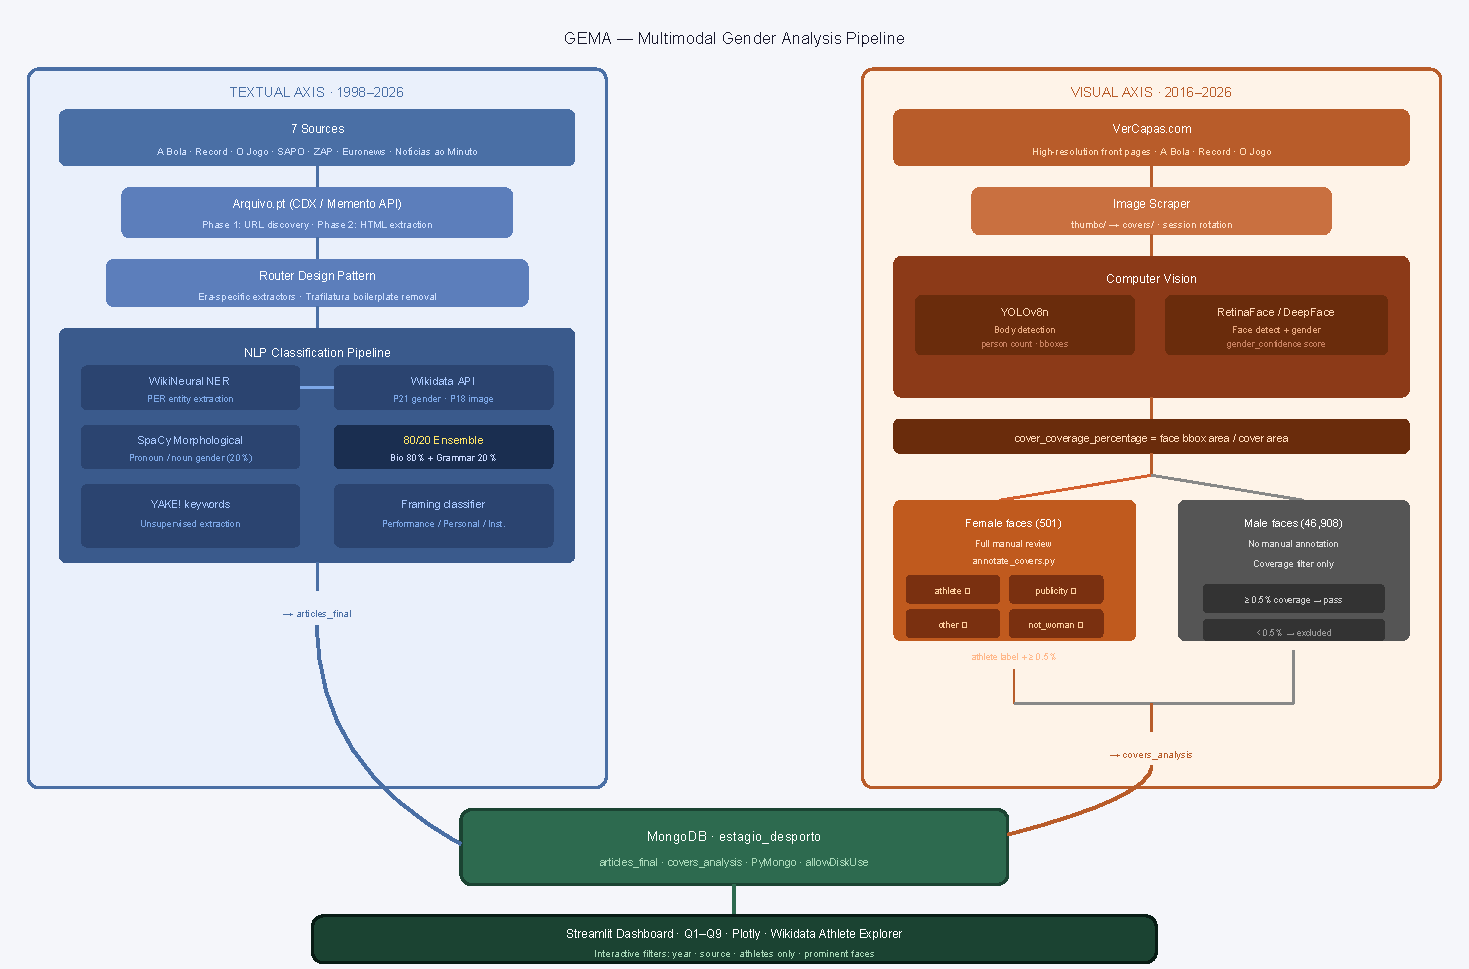
\includegraphics[width=\textwidth]{figures/architecture.pdf}
  \caption{High-level architecture of the GEMA pipeline. Both axes write to a shared MongoDB instance (\texttt{estagio\_desporto}), which feeds the Streamlit analytical dashboard.}
  \label{fig:architecture}
\end{figure}

\begin{table}[H]
\centering
\caption{Web technology eras handled by the Router Design Pattern.}
\label{tab:eras}
\begin{tabularx}{\textwidth}{llX}
\toprule
\textbf{Period} & \textbf{Technology} & \textbf{Extraction strategy} \\
\midrule
1998–2005 & Static HTML (tables, \texttt{<font>}) & Tag-based heuristics \\
2005–2012 & ASP.NET dynamic pages & Form-aware BeautifulSoup \\
2012–2018 & CMS-based (WordPress, Drupal) & Semantic CSS selectors (BeautifulSoup) \\
2018–2026 & SPA (Next.js, React) & Direct API / BeautifulSoup fallback \\
\bottomrule
\end{tabularx}
\end{table}

\begin{table}[H]
\centering
\caption{Comparison of the five gender classification approaches evaluated during the internship. The 80/20 WikiNeural weighted ensemble was selected for production.}
\label{tab:model_comparison}
\begin{tabularx}{\textwidth}{Xp{1.6cm}p{2.8cm}p{2.4cm}p{1.6cm}}
\toprule
\textbf{Approach} & \textbf{Speed} & \textbf{False positives} & \textbf{Ambiguity handling} & \textbf{Cost} \\
\midrule
Lexical (census)        & Very fast & High (gramm.\ FP) & None      & Free \\
Stanza~\cite{Stanza} / SpaCy~\cite{SpaCy} & Fast & Medium & Partial & Free \\
WikiNeural~\cite{Tedeschi2021} (NER) & Medium & Low & Partial & Free \\
mDeBERTa-v3~\cite{mDeBERTa} & Medium & Low & Good & Free \\
GPT-4o                  & Slow      & Very low          & Excellent & API cost \\
\textbf{80/20 ensemble} & Medium    & \textbf{Very low} & \textbf{Good} & Low \\
\bottomrule
\end{tabularx}
\end{table}

% ── Q figures ─────────────────────────────────────────────────────────────────
\begin{figure}[H]
  \centering
  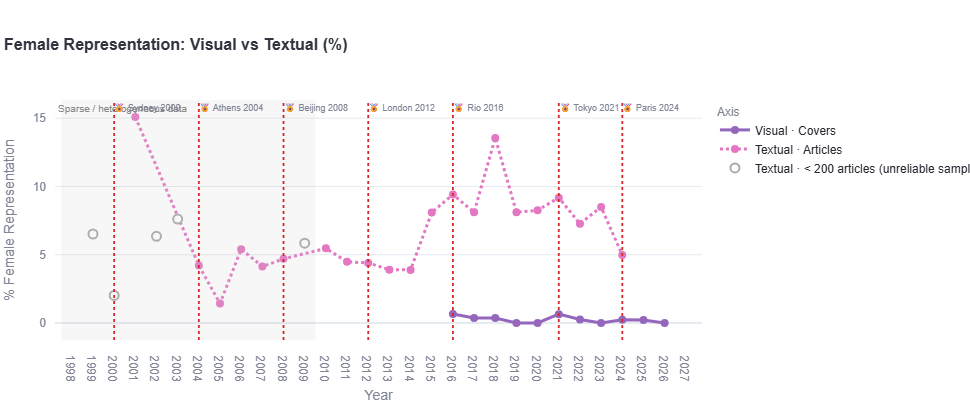
\includegraphics[width=0.6\textwidth]{figures/q1_evolution.png}
  \caption{\textbf{Q1 —} Annual female representation (\%) on the textual axis (dashed pink, 1998--2024) and visual axis (solid purple, 2016--2026). Olympic years are marked by red vertical dashed lines; open circles indicate fewer than 200 articles that year. Spikes that vanish the following year signal a temporary event effect rather than structural change.}
  \label{fig:q1}
\end{figure}

  \vspace{1em}

\begin{figure}[H]
  \centering
  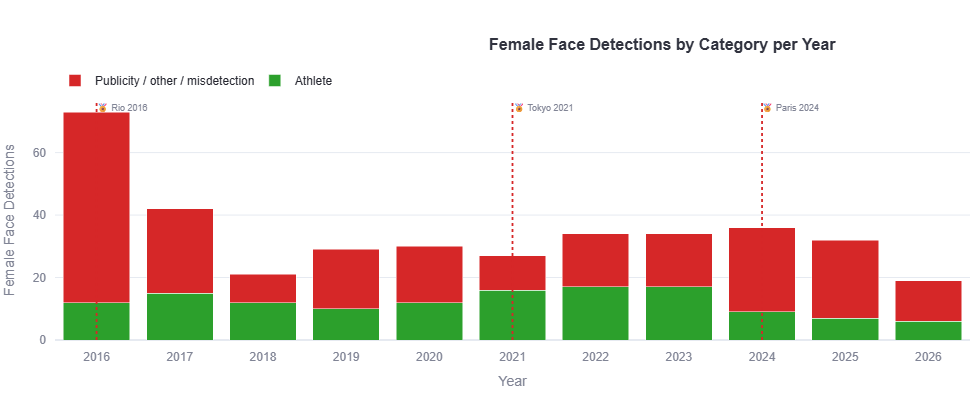
\includegraphics[width=0.6\textwidth]{figures/q2_false_positives.png}
  \caption{\textbf{Q2 —} Stacked bar chart of female face detections per year (2016--2026): green = confirmed athletes, red = advertising models, fans, or gender misdetections. Olympic years are marked. A tall green bar means the event genuinely brought more female athletes to covers; a predominantly red bar means most detections that year were not athletes.}
  \label{fig:q2}
\end{figure}

\begin{figure}[H]
  \centering
  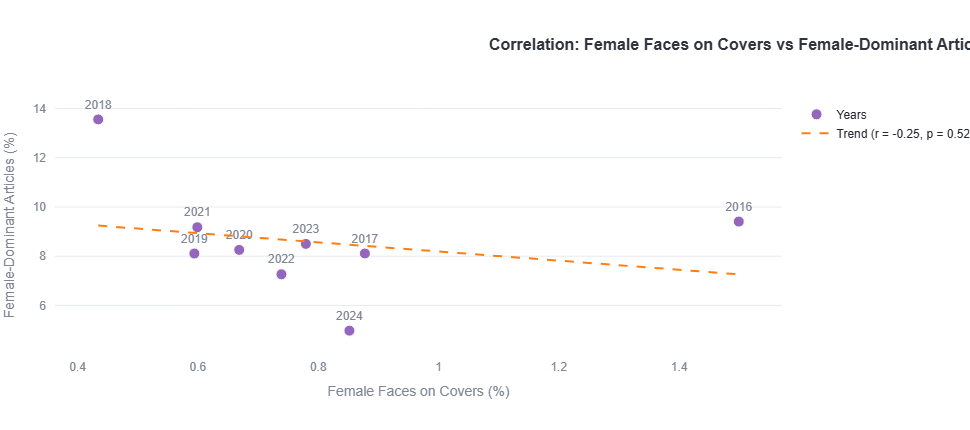
\includegraphics[width=0.6\textwidth]{figures/q3_sources_a.png}
  \caption{\textbf{Q3a —} Scatter plot of annual visual-axis female \% (x) vs.\ textual-axis female \% (y) for each year 2016--2026. Each dot is a labelled year; OLS trend line and Pearson $r$ are shown. Points clustering along a rising diagonal would indicate the two channels move together; flat or downward scatter means they are editorially independent.}
  \label{fig:q3a}
\end{figure}

  \vspace{1em}

\begin{figure}[H]
  \centering
  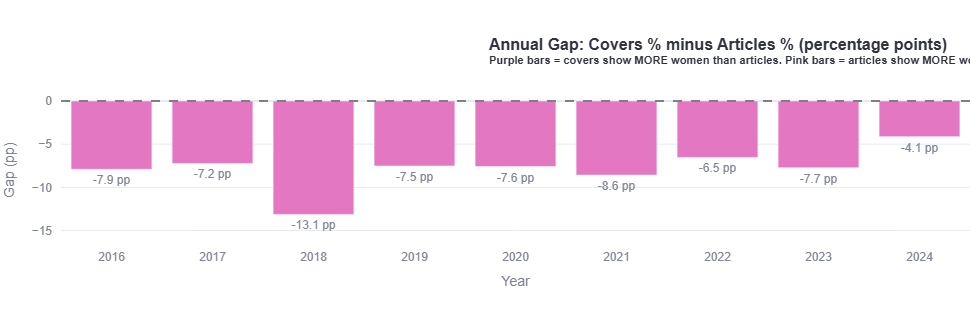
\includegraphics[width=0.6\textwidth]{figures/q3_sources_b.png}
  \caption{\textbf{Q3b —} Annual gap in percentage points (cover female \% $-$ article female \%) for 2016--2024. All bars are negative, meaning the textual axis always shows more women than the visual axis. A more negative bar = a wider disconnect between article writers and cover editors that year.}
  \label{fig:q3b}
\end{figure}

\begin{figure}[H]
  \centering
  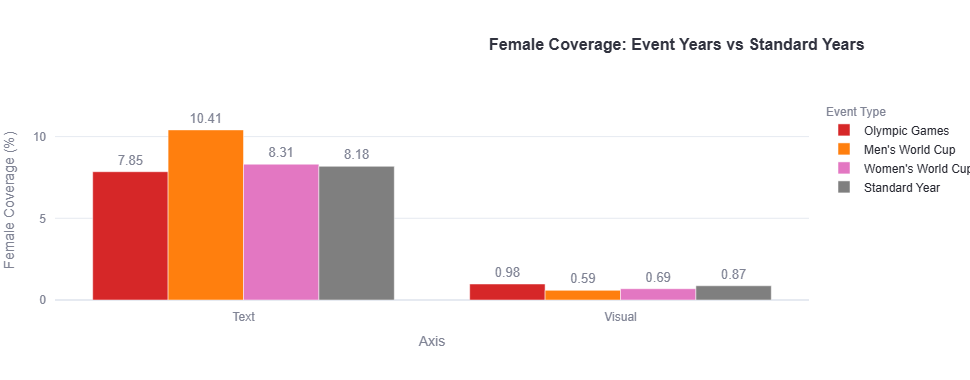
\includegraphics[width=0.6\textwidth]{figures/q4_events.png}
  \caption{\textbf{Q4 —} Grouped bar chart of mean female coverage (\%) by event-year type (Standard / Olympic / Men's WC / Women's WC), for both the textual and visual axes. Mann-Whitney U $p$-values are shown. Taller bars = higher average female representation in those event years; similar bar heights across groups = no statistically significant event boost.}
  \label{fig:q4}
\end{figure}

  \vspace{1em}

\begin{figure}[H]
  \centering
  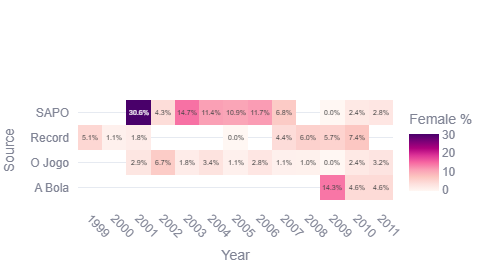
\includegraphics[width=0.6\textwidth]{figures/q5_heatmap_a.png}
  \caption{\textbf{Q5a —} Heatmap of female article coverage (\%) by source (rows) and year (columns), 1999--2011. Darker cells = higher representation; white/missing = fewer than 10 articles. A consistently dark row means the outlet systematically covers more women; an isolated dark cell in an otherwise light row indicates an event-driven spike.}
  \label{fig:q5a}
\end{figure}
  
\begin{figure}[H]
  \centering
  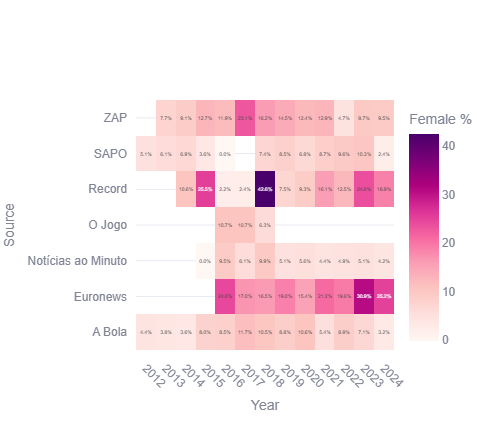
\includegraphics[width=0.6\textwidth]{figures/q5_heatmap_b.png}
  \caption{\textbf{Q5b —} Heatmap of female article coverage (\%) by source and year, 2012--2024 (same colour scale as Figure~\ref{fig:q5a}). Comparing rows reveals which outlets systematically under- or over-represent women; comparing columns shows event-driven year spikes across all sources simultaneously.}
  \label{fig:q5b}
\end{figure}

  \vspace{1em}

\begin{figure}[H]
  \centering
  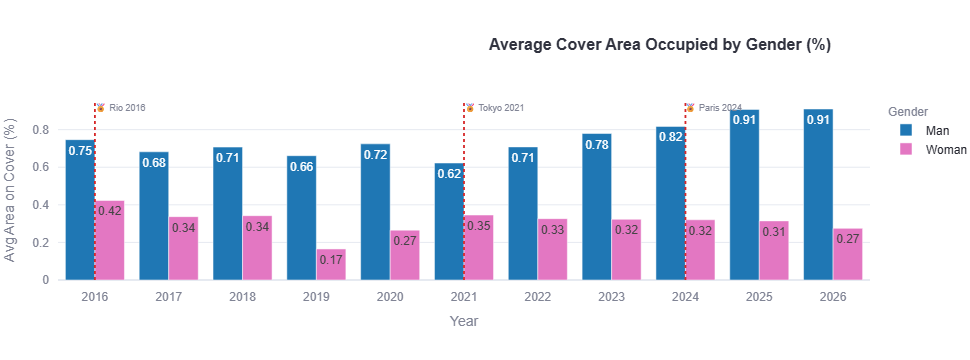
\includegraphics[width=0.6\textwidth]{figures/q6_prominence_a.png}
  \caption{\textbf{Q6a —} Mean cover area (\%) occupied by male (blue) vs.\ female (pink) athlete faces per year. Taller blue bars mean male athletes receive more page space that year; years where pink approaches blue indicate greater spatial parity.}
  \label{fig:q6a}
\end{figure}

\begin{figure}[H]
  \centering
  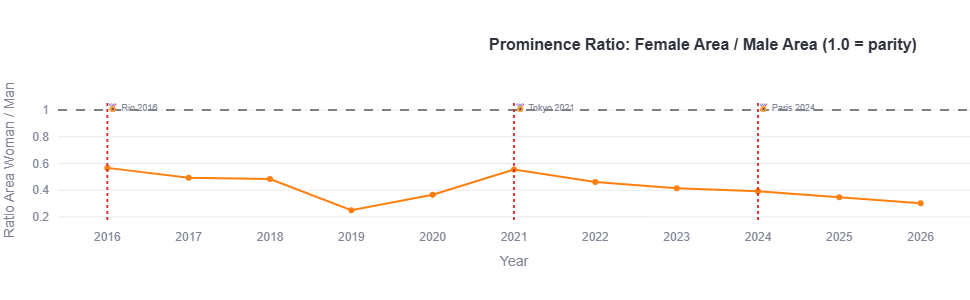
\includegraphics[width=0.6\textwidth]{figures/q6_prominence_b.png}
  \caption{\textbf{Q6b —} Annual prominence ratio (female mean cover area / male mean cover area). The dashed horizontal line at 1.0 = full parity; values below 1.0 mean male faces are visually larger on average. Olympic years are marked. A ratio near 1.0 means cover editors gave female athletes the same page space as male athletes that year.}
  \label{fig:q6b}
\end{figure}

  \vspace{1em}

\begin{figure}[H]
  \centering
  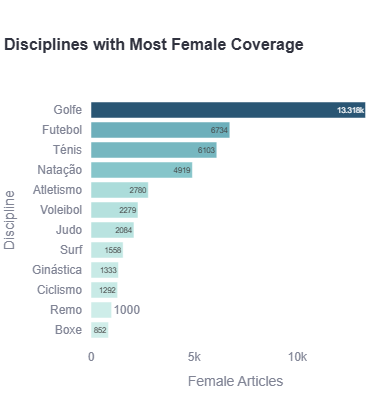
\includegraphics[width=0.6\textwidth]{figures/q7_disciplines_a.png}
  \caption{\textbf{Q7a —} Total female-protagonist articles per sports discipline across all years, sorted descending. A longer bar means more cumulative coverage in that discipline; the ranking may differ from what is expected based on the sport's general prominence.}
  \label{fig:q7a}
\end{figure}

\begin{figure}[H]
  \centering
  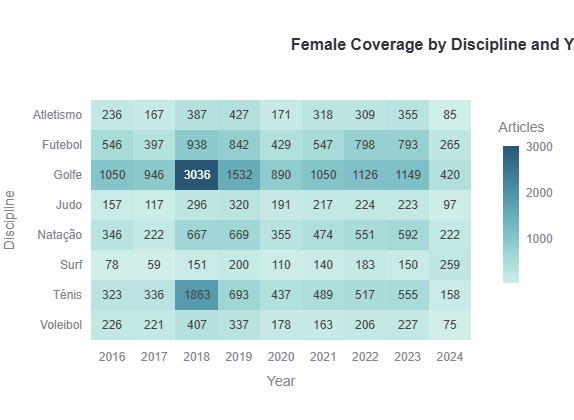
\includegraphics[width=0.6\textwidth]{figures/q7_disciplines_b.png}
  \caption{\textbf{Q7b —} Heatmap of female-protagonist articles per discipline (rows) and year (columns), 2016--2024. A shared color scale enables direct cross-discipline comparison. Consistently dark rows indicate sustained coverage; isolated dark cells indicate event-year spikes.}
  \label{fig:q7b}
\end{figure}

  \vspace{1em}

\begin{figure}[H]
  \centering
  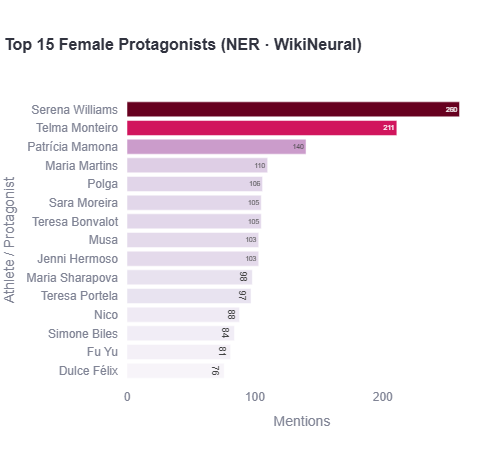
\includegraphics[width=0.6\textwidth]{figures/q8_diversity_a.png}
  \caption{\textbf{Q8a —} Top 15 female protagonists by total NER mention count across 1998--2024. A longer bar means more cumulative articles; the gap between consecutive bars shows whether coverage is concentrated in a few stars or distributed across a broader pool.}
  \label{fig:q8a}
\end{figure}

\begin{figure}[H]
  \centering
  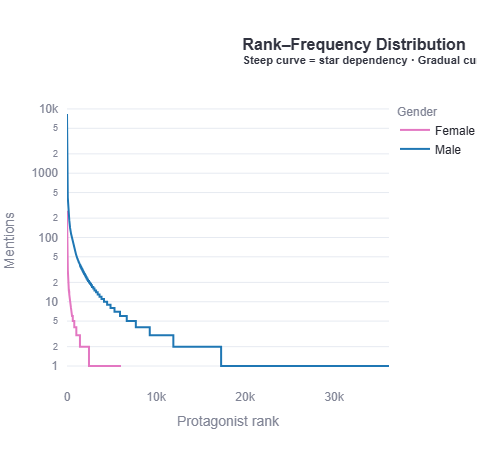
\includegraphics[width=0.6\textwidth]{figures/q8_diversity_b.png}
  \caption{\textbf{Q8b —} Rank-frequency distribution (log y-axis) for female (pink) and male (blue) protagonist pools. Rank 1 = most mentioned athlete. A curve that drops steeply and ends early indicates a shallow pool concentrated in a few stars; a long gradual tail means coverage extends to many athletes.}
  \label{fig:q8b}
\end{figure}

  \vspace{1em}

\begin{figure}[H]
  \centering
  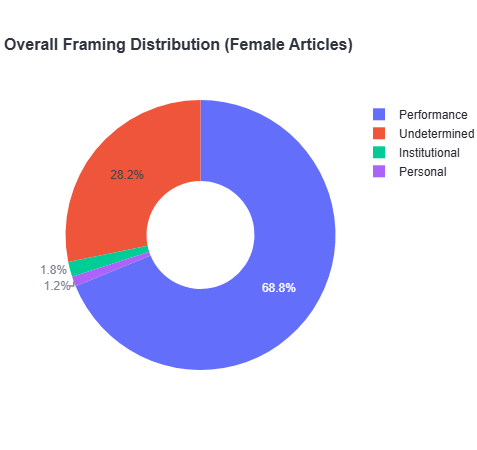
\includegraphics[width=0.6\textwidth]{figures/q9_semantic_a.png}
  \caption{\textbf{Q9a —} Donut chart of framing category distribution across all female-dominant articles: Performance (victories, records, medals), Undetermined (fewer than 2 keyword matches), Institutional (governance, federation), Personal (family, relationships). A dominant Performance segment is a positive sign; a large Undetermined segment indicates many articles are too brief to classify reliably.}
  \label{fig:q9a}
\end{figure}

\begin{figure}[H]
  \centering
  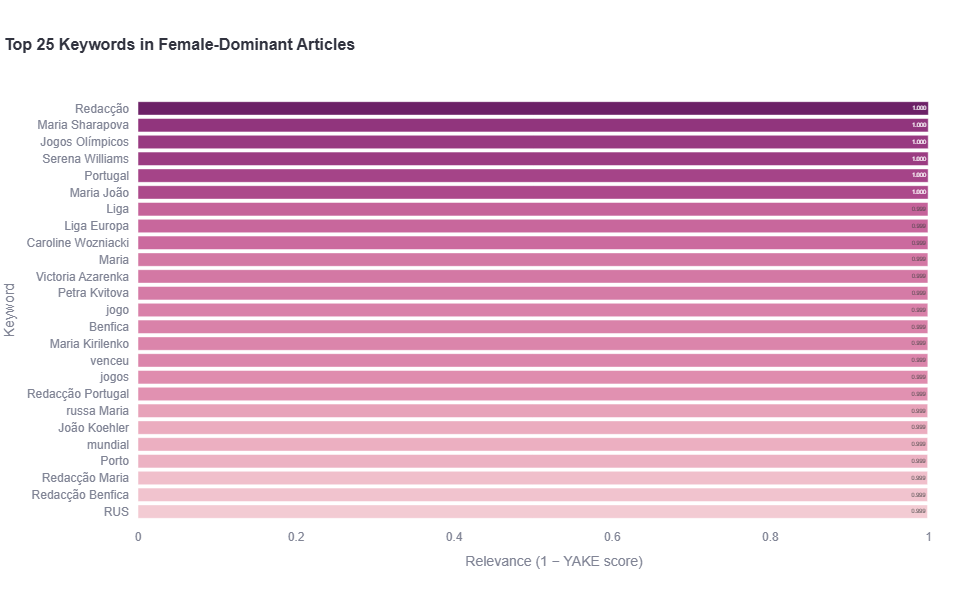
\includegraphics[width=\textwidth]{figures/q9_semantic_b.png}
  \caption{\textbf{Q9b —} Top 25 YAKE!-extracted bi-gram keywords from female-dominant articles, sorted by normalised relevance (1~$-$~YAKE score; longer bar = more characteristic of this corpus). Athlete names at the top indicate star-dominated coverage; competition terms indicate performance-focused framing.}
  \label{fig:q9b}
\end{figure}

\end{document}
